\subsection{Linux features}

\begin{frame}
  \frametitle{History}
  \begin{columns}
    \column{0.8\textwidth}
    \begin{itemize}
    \item The Linux kernel is one component of a system, which also
      requires libraries and applications to provide features to end
      users.
    \item The Linux kernel was created as a hobby in 1991 by a Finnish
      student, Linus Torvalds.
      \begin{itemize}
      \item Linux quickly started to be used as the kernel for free
        software operating systems
      \end{itemize}
    \item Linus Torvalds has been able to create a large and dynamic
      developer and user community around Linux.
    \item Nowadays, more than one thousand people contribute to each kernel
      release, individuals or companies big and small.
    \end{itemize}
    \column{0.2\textwidth}
      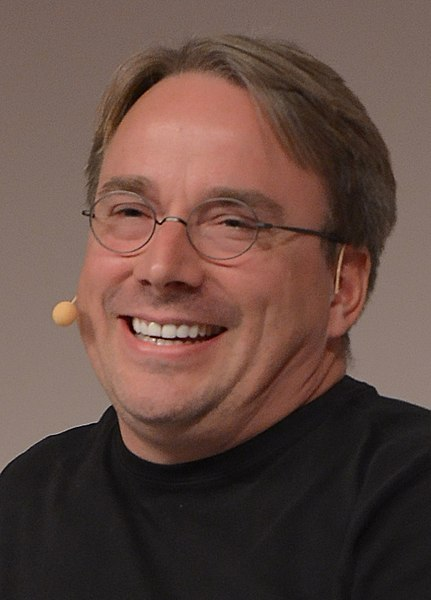
\includegraphics[width=\textwidth]{slides/sysdev-linux-intro-features/linus-torvalds.jpg}
      \scriptsize
      Linus Torvalds in 2014\\
      \tiny
      Image credits (Wikipedia):\\
      \url{https://bit.ly/2UIa1TD}
    \end{columns}
\end{frame}

\begin{frame}
  \frametitle{Linux kernel key features}
  \begin{columns}
    \column{0.5\textwidth}
    \begin{itemize}
    \item Portability and hardware support. Runs on most
      architectures.
    \item Scalability. Can run on super computers as well as on tiny
      devices (4 MB of RAM is enough).
    \item Compliance to standards and interoperability.
    \item Exhaustive networking support.
    \end{itemize}
    \column{0.5\textwidth}
    \begin{itemize}
    \item Security. It can't hide its flaws. Its code is reviewed by
      many experts.
    \item Stability and reliability.
    \item Modularity. Can include only what a system needs even at run
      time.
    \item Easy to program. You can learn from existing code. Many
      useful resources on the net.
    \end{itemize}
  \end{columns}
\end{frame}

\begin{frame}
  \frametitle{Linux kernel in the system}
  \begin{center}
    \includegraphics[height=0.8\textheight]{slides/sysdev-linux-intro-features/linux-kernel-in-system.pdf}
  \end{center}
\end{frame}

\begin{frame}{Linux kernel main roles}
  \begin{itemize}
  \item {\bf Manage all the hardware resources}: CPU, memory, I/O.
  \item Provide a {\bf set of portable, architecture and hardware
      independent APIs} to allow user space applications and libraries
    to use the hardware resources.
  \item {\bf Handle concurrent accesses and usage} of hardware
    resources from different applications.
    \begin{itemize}
    \item Example: a single network interface is used by multiple
      user space applications through various network connections. The
      kernel is responsible to ``multiplex'' the hardware resource.
    \end{itemize}
  \end{itemize}
\end{frame}

\begin{frame}
  \frametitle{System calls}
  \begin{columns}
    \column{0.7\textwidth}
    \begin{itemize}
    \item The main interface between the kernel and user space is the set
      of system calls
    \item About 400 system calls that provide the main kernel services
      \begin{itemize}
      \item File and device operations, networking operations,
        inter-process communication, process management, memory mapping,
        timers, threads, synchronization primitives, etc.
      \end{itemize}
    \item This interface is stable over time: only new system calls can
      be added by the kernel developers
    \item This system call interface is wrapped by the C library, and
      user space applications usually never make a system call directly
      but rather use the corresponding C library function
    \end{itemize}
    \column{0.3\textwidth}
      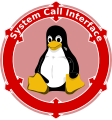
\includegraphics[width=\textwidth]{slides/sysdev-linux-intro-features/system-calls.pdf}
      \scriptsize
      Image credits (Wikipedia):\\
      \url{https://bit.ly/2U2rdGB}
    \end{columns}
\end{frame}

\begin{frame}
  \frametitle{Pseudo filesystems}
  \begin{itemize}
  \item Linux makes system and kernel information available in user
    space through {\bf pseudo filesystems}, sometimes also called {\bf
      virtual filesystems}
  \item Pseudo filesystems allow applications to see directories and
    files that do not exist on any real storage: they are created and
    updated on the fly by the kernel
  \item The two most important pseudo filesystems are
    \begin{itemize}
    \item \code{proc}, usually mounted on \code{/proc}: \\
      Operating system related information (processes, memory
      management parameters...)
    \item \code{sysfs}, usually mounted on \code{/sys}: \\
       Representation of the system as a set of
       devices and buses. Information about these devices.
    \end{itemize}
  \end{itemize}
\end{frame}

\begin{frame}{Inside the Linux kernel}
  \begin{center}
    \includegraphics[width=\textwidth]{slides/sysdev-linux-intro-features/inside-linux-kernel.pdf}
  \end{center}
\end{frame}

\expandafter\ifstrequal\expandafter{\training}{kernel}{}
{
\begin{frame}
  \frametitle{Linux license}
  \begin{itemize}
  \item The whole Linux sources are Free Software released under the
    GNU General Public License version 2 (GPL v2).
  \item For the Linux kernel, this basically implies that:
    \begin{itemize}
    \item When you receive or buy a device with Linux on it, you
      should receive the Linux sources, with the right to study,
      modify and redistribute them.
    \item When you produce Linux based devices, you must release the
      sources to the recipient, with the same rights, with no
      restriction.
    \end{itemize}
  \end{itemize}
\end{frame}
}

\begin{frame}
  \frametitle{Supported hardware architectures}
  See the \kdir{arch} directory in the kernel sources
  \begin{itemize}
  \item Minimum: 32 bit processors, with or without MMU, and
    \code{gcc} support
  \item 32 bit architectures (\kdir{arch} subdirectories)\\
    Examples: \ksubarch{arm}, \ksubarch{arc},
    \ksubarch{c6x}, \ksubarch{m68k}, \ksubarch{microblaze}...
  \item 64 bit architectures:\\
    Examples: \ksubarch{alpha}, \ksubarch{arm64}, \ksubarch{ia64}...
  \item 32/64 bit architectures\\
    Examples: \ksubarch{mips}, \ksubarch{powerpc}, \ksubarch{riscv}, \ksubarch{sh},
              \ksubarch{sparc}, \ksubarch{x86}...
  \item Note that unmaintained architectures can also be removed when they have compiling issues and nobody fixes them.
  \item Find details in kernel sources: \code{arch/<arch>/Kconfig},
    \code{arch/<arch>/README}, or \code{Documentation/<arch>/}
  \end{itemize}
\end{frame}
